\subsection{Simulador del Physarum Polycephalum} % (fold)
\label{sub:subsection name}

    El algoritmo propuesto se basa en el descrito por Jeff Jones en su obra 
    'From Pattern Formation to Material Computation: Multi-agent Modelling of Physarum Polycephalum' \cite{Jones2015}.
    \vskip 0.5cm
    %P\'arrafo 2
    El algoritmo es un aut\'omata celular que simula el comportamiento de Physarum Polycephalum en un laberinto, por lo que necesitamos definir algunos conceptos.
        Primero, denotemos $\mathbb{Z}$ como el conjunto de enteros, es decir, $\mathbb{Z} = (-\infty, -1, 0, 1, \infty)$.
        y la longitud de cualquier tupla $x$ como $|x|$. Para todas las tuplas $x$ e $y$ de la misma longitud, denotemos $x \oplus y$
        como la tupla que resulta de la suma componente a componente de $x$ e $y$, es decir, $(x \oplus y)_i = x_i + y_i$ para todo
    $i \in \mathbb{Z}$.
    \vskip 0.5cm
    %P\'arrafo 3
    Entonces tenemos que un aut\'omata celular es una tupla $(\mathbb{Z}^{n}, S, N, f)$ tal que la dimensi\'on $n$ es al menos 1 donde 
        $n \in \mathbb{Z}^{+}$, $S$ es un conjunto finito y no vac\'io de estados, $N$ es un conjunto finito y no vac\'io de vecindarios 
        pertenecientes a $\mathbb{Z}^{n}$, y $f$ es una funci\'on de transici\'on local, es decir, $f: S^N \rightarrow S$ donde
        $S^N$ representa el conjunto de todas las configuraciones de vecindarios posibles en $N$.
    \vskip 0.5cm
    %P\'arrafo 4
    As\'i, el algoritmo propuesto en este trabajo se define como un aut\'omata celular $(\mathbb{Z}^{2}, S, N, f)$ donde $n = 2$, 
        $S = \{0, 1, 2, 3, 4, 5, 6, 7, 8\}$, $N = \{0, 1, 2, 3, 4, 5, 6, 7, 8\}^9$, 
        y $f : \{0, 1, 2, 3, 4, 5, 6, 7, 8\}^9 \rightarrow \{0, 1, 2, 3, 4, 5, 6, 7, 8\}$,\((C(x,y:t), N(x,y:t), M(x,y:t)) \) 
        representa el estado combinado, vecindario y memoria de la c\'elula en la posici\'on \((x, y)\) en el tiempo \( t \). La funci\'on de transici\'on 
        \( f \) se define como sigue:
    \begin{equation*}
    \begin{aligned}
    f(C(x,y:t), N(x,y:t), M(x,y:t)) = & \begin{cases}
        7 & \text{si } C(x,y:t) = 0 \text{ y } \exists N \in \{3, 4, 6\} \text{y } M(x,y:t) = 0 \\
        6 & \text{si } C(x,y:t) = 1 \text{ y } \exists N \in \{5, 6\} \\
        2 & \text{si } C(x,y:t) = 2 \\
        3 & \text{si } C(x,y:t) = 3 \\
        5 & \text{si } C(x,y:t) = 4 \text{ y } \exists N \in \{3, 5, 6\} \\
        & \text{y } M(x,y:t) = 0 \text{ y } N \not\in \{0, 7\} \\
        0 & \text{si } C(x,y:t) = 5 \text{ y } M(x,y:t) \not\in \{5, 8\} \\
        & \text{y } N \not\in \{1, 3, 4, 6\} \\
        8 & \text{si } C(x,y:t) = 5 \\
        & \text{ y la condici\'on anterior no se cumple} \\
        4 & \text{si } C(x,y:t) = 7 \text{ y } \exists N \in \{3, 4, 6\} \\
        5 & \text{si } C(x,y:t) = 8 \\
        1 & \text{si } C(x,y:t) = 1 \\
    \end{cases}
    \end{aligned}
    \end{equation*}
    %Tabla de estados
    Donde los estados del aut\'omata celular se definen en la \textbf{Tabla \ref{tab:estados}}.
    \vskip 0.5cm
    \begin{table}[h]
        \begin{center}
            \begin{tabular}{|c|c|c|}
                \hline
                \textbf{Color}&\textbf{Estado}&\textbf{Descripci\'on} \\
                \hline
                \cellcolor{blue} & 0 & Campo libre  \\
                \cellcolor{royalblue} & 1 & Nutriente no encontrado \\
                \cellcolor{red} & 2 & Repelente \\
                \cellcolor{black} & 3 & Punto inicial \\
                \cellcolor{yellow} & 4 & Gel contray\'endose \\
                \cellcolor{darkgreen} & 5 & Gel compuesto \\
                \cellcolor{lemon} & 6 & Nutriente encontrado \\
                \cellcolor{darkgray} & 7 & Expansi\'on de Physarum \\
                \cellcolor{green} & 8 & Gel no compuesto \\
                \hline
            \end{tabular}
        \end{center}
        \caption{Estados del aut\'omata celular}
        \label{tab:estados}
    \end{table}
    \begin{table}[h]
        \begin{center}
            \begin{tabular}{|c|c|c|}
                \hline
                \textbf{Color}&\textbf{State}&\textbf{Initial State Catacomb} \\
                \hline
                \cellcolor{blue} & 0 & 32,891  \\
                \cellcolor{royalblue} & 1 & 1 \\
                \cellcolor{red} & 2 & 967,105 \\
                \cellcolor{black} & 3 & 2 \\
                \cellcolor{yellow} & 4 & 0 \\
                \cellcolor{darkgreen} & 5 & 0 \\
                \cellcolor{lemon} & 6 & 0 \\
                \cellcolor{darkgray} & 7 & 0 \\
                \cellcolor{green} & 8 & 0 \\
                \hline
            \end{tabular}
        \end{center}
        \caption{Estados del aut\'omata celular}
        \label{tab:estados}
    \end{table}
    \begin{table}[h]
        \begin{center}
            \begin{tabular}{|c|c|c|}
                \hline
                \textbf{Color}&\textbf{State}&\textbf{Initial State Cave} \\
                \hline
                \cellcolor{blue} & 0 & 853,861  \\
                \cellcolor{royalblue} & 1 & 3 \\
                \cellcolor{red} & 2 & 146,135 \\
                \cellcolor{black} & 3 & 1 \\
                \cellcolor{yellow} & 4 & 0 \\
                \cellcolor{darkgreen} & 5 & 0 \\
                \cellcolor{lemon} & 6 & 0 \\
                \cellcolor{darkgray} & 7 & 0 \\
                \cellcolor{green} & 8 & 0 \\
                \hline
            \end{tabular}
        \end{center}
        \caption{Estados del aut\'omata celular}
        \label{tab:estados}
    \end{table}
    \vskip 0.5cm
    %P\'arrafo x
    En la fuente mencionada, se detalla el algoritmo b\'asico de Physarum Polycephalum, dise\~nado originalmente para operar con un vecindario de Von 
        Neumann. Sin embargo, en la versi\'on propuesta aqu\'i, optamos por modificar el vecindario a uno de Moore, 
        facilitando as\'i el acceso a un mayor n\'umero de vecinos para comparaci\'on y permitiendo obtener una perspectiva m\'as clara de la direcci\'on \'optima 
        para el desplazamiento del agente.
    Sin embargo, el uso del vecindario de Moore en lugar del vecindario de Von Neumann introduce ciertos desaf\'ios no presentes en el algoritmo original. 
        Uno de estos desaf\'ios surge en las esquinas (NW, NE, SW, SE), donde el repelente podr\'ia permitir que el agente escape, 
        contrario a lo deseado. Para abordar este inconveniente, se implement\'o una soluci\'on que consiste en colocar un repelente imaginario en la esquina cuando 
        dos esquinas adyacentes presentan repelentes en un \'angulo de 90\degree  entre s\'i. Este ajuste permite la creaci\'on de una gama m\'as amplia de formas, 
        como se ilustra en las Figs \ref{fig:physarumCircle1}, 
        \ref{fig:physarumRandom1} y \ref{fig:physarumObstacles1}. En estas im\'agenes, el n\'umero total de c\'elulas es de 50 x 50.
    \vskip 0.5cm
    \begin{figure}[htbp]
        \centerline{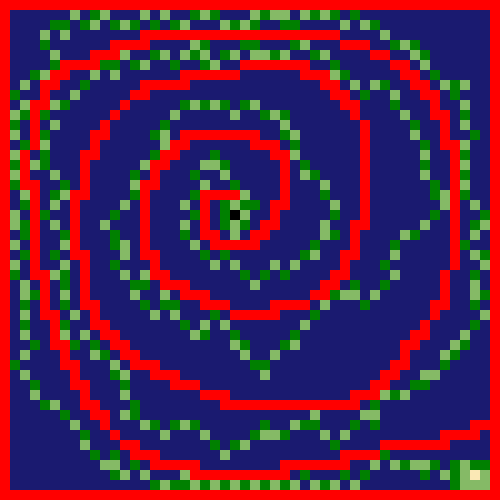
\includegraphics[width=0.5\textwidth]{./images/desarrollo/physarum/Circular1.png}}
        \caption{Physarum Polycephalum resolviendo un laberinto en espiral.} 
        \label{fig:physarumCircle1}    
    \end{figure}
    \begin{figure}[htbp]
        \centerline{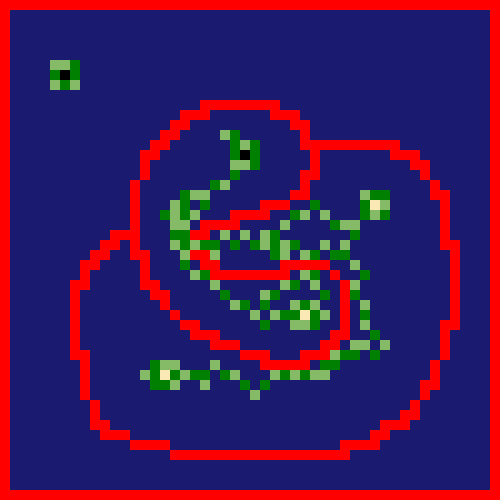
\includegraphics[width=0.5\textwidth]{./images/desarrollo/physarum/Random1.png}}
        \caption{Physarum Polycephalum resolviendo un laberinto de tipo circular.}
        \label{fig:physarumRandom1}    
    \end{figure}
    \begin{figure}[htbp]
        \centerline{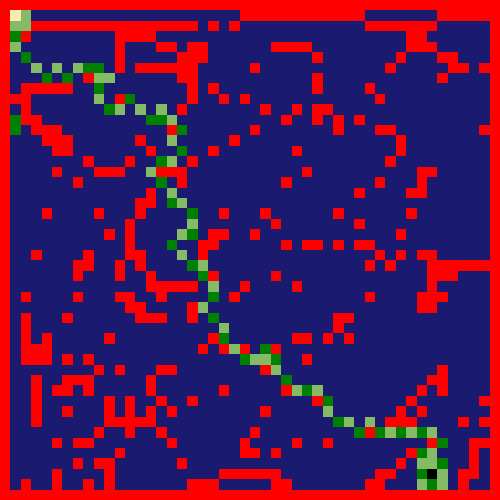
\includegraphics[width=0.5\textwidth]{./images/desarrollo/physarum/Obstaculos1.png}}
        \caption{Physarum Polycephalum resolviendo un laberinto con obst\'aculos.}
        \label{fig:physarumObstacles1}
    \end{figure}
    \vskip 0.5cm
    %P\'arrafo 3
    Gracias a la resoluci\'on de la fuga en las esquinas por nuestro algoritmo, es posible generar mapeos m\'as diversos 
        de cuevas y catacumbas. Este enfoque mejora significativamente nuestra comprensi\'on 
        de la topograf\'ia del \'area explorada. Adem\'as, la diversidad en el mapeo facilita la identificaci\'on 
        del n\'umero y variedad de caminos disponibles, lo que se ha implementado mediante un algoritmo de mapeo de im\'agenes que 
        ayuda en la representaci\'on gr\'afica de dicha topograf\'ia, como se muestra en la Fig \ref{fig:CaveSystemPhysarum}.
    \vskip 0.5cm
        \begin{figure}[htbp]
            \centerline{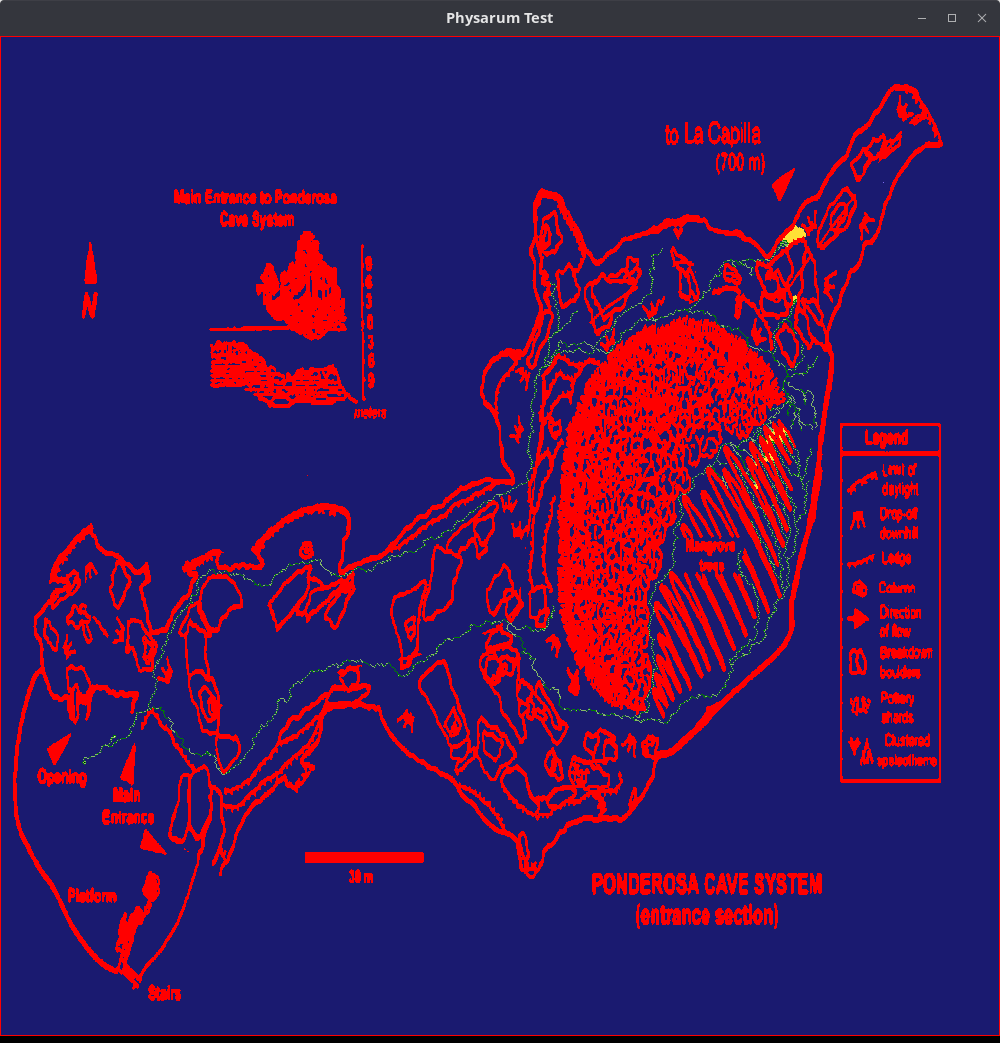
\includegraphics[width=0.40\textwidth]{./images/desarrollo/physarum/CaveSystemPhysarum.png}}
            \caption{Mapeo del sistema de cuevas usando Physarum Polycephalum.}
            \label{fig:CaveSystemPhysarum}
        \end{figure}
        \vskip 0.2cm
        Tambi\'en el algoritmo ha sido probado en un entorno real, donde ha sido capaz de generar 
            rutas \'optimas en la Catacumba de Par\'is, como se muestra en la Fig \ref{fig:Catacomb}. El espacio
            explorado por el algoritmo es de 1000 x 1000 c\'elulas.
        \vskip 0.2cm
        \begin{figure}[htbp]
            \centerline{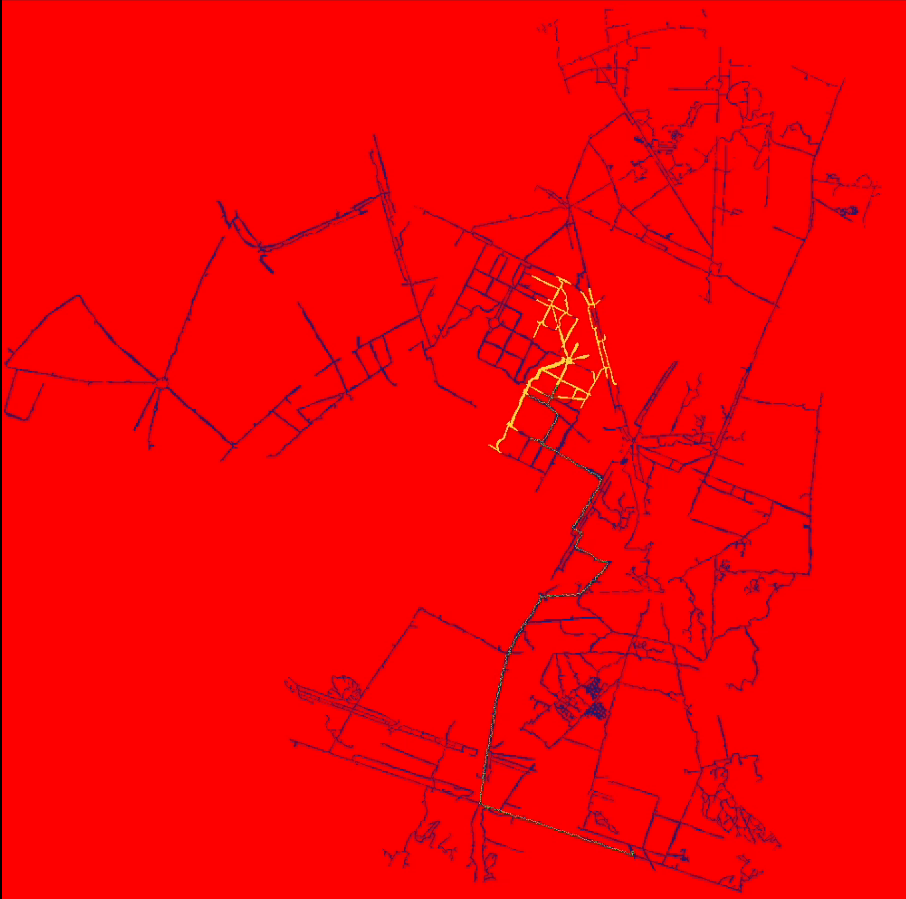
\includegraphics[width=0.40\textwidth]{./images/desarrollo/physarum/CatacoumbParis.png}}
            \caption{Mapeo de la catacumba usando Physarum Polycephalum, utiliza 5264 pasos para obtener la ruta.}
            \label{fig:Catacomb}
        \end{figure}
        %P\'arrafo 4
        Cabe se\~nalar que dado que el algoritmo est\'a bioinspirado, la funci\'on que simula el comportamiento del plasmodio 
            se asigna de manera pseudoaleatoria a un vecino adyacente, con una probabilidad de 1/8. Esta caracter\'istica permite 
            que la expansi\'on del algoritmo tome una forma circular en lugar de una expansi\'on cuadrada o lineal. Sin embargo, al 
            modificar la funci\'on de probabilidad, es posible lograr una expansi\'on m\'as irregular en lugar de simplemente circular.
        \clearpage
        En cuanto la implementaci\'on del algoritmo, se ha utilizado el lenguaje de programaci\'on C++ y la librer\'ia OpenCV para la 
            obtenci\'on de im\'agenes. La parte de las esquinas que mencionamos con anterioridad se implement\'o de la siguiente manera: 
        \begin{lstlisting}[language={C++}, caption={Implementaci\'on del problema de las esquinas}, label={Script}]
            std::vector<int> Physarum::isOnCorner(std::vector<int> neighboursData) {
            std::vector<int> corners;
                if (neighboursData[0] == 2 && neighboursData[2] == 2) {
                    corners.push_back(1);
                }
                if (neighboursData[0] == 2 && neighboursData[6] == 2) {
                    corners.push_back(7);
                }
                if (neighboursData[6] == 2 && neighboursData[4] == 2) {
                    corners.push_back(5);
                }
                if (neighboursData[2] == 2 && neighboursData[4] == 2) {
                    corners.push_back(3);
                }
            return corners;
            }
        \end{lstlisting}
        %P\'arrafo 5
        En el c\'odigo \ref{Script}, se muestra la implementaci\'on de la funci\'on que detecta si el agente se encuentra en una esquina. 
            La funci\'on recibe un vector de enteros que representa los estados de los vecinos adyacentes. Si dos esquinas adyacentes 
            presentan repelentes, la funci\'on devuelve un vector con las esquinas en las que se encuentra el agente. 
            En caso contrario, la funci\'on devuelve un vector vac\'io.
        \vskip 0.5cm
        %P\'arrafo 6
        Por ello podemos decir que el algoritmo propuesto es capaz de resolver laberintos de manera eficiente, 
            generando rutas \'optimas en entornos complejos y desconocidos. Adem\'as, el algoritmo es capaz de 
            adaptarse a diferentes topograf\'ias, lo que lo convierte en una herramienta vers\'atil para la exploraci\'on 
            de entornos desconocidos y nos es de ayuda en el monitoreo de poblaciones y sistemas relacionados.
        \vskip 0.5cm
        
% subsection subsection name (end)